\section{Nodal Coordinate and Element Connections}

The basic mesh for {\sl FEAPpv} consists of nodes and elements.
For the general finite elements included with the program the mesh
is described relative to a global Cartesian coordinate frame.  For
two-dimensional plane problems the mesh lies in the $x_1$-$x_2$ plane
(or the $x-y$ plane).  For axisymmetric problems the mesh lies in the
$r-z$ plane (which is placed in the $x_1$-$x_2$ plane).  For three
dimensional problems a general $x_1$, $x_2$, $x_3$ (or $x$, $y$, $z$)
coordinate system is used.  In the sequel we will discuss the specification
of the input data relative to the $x_i$ components.  While eventually all
nodal coordinates must be specified relative to the $x_i$ frame, it is
possible to use other coordinate systems (e.g., polar and spherical)
as the input data and
then transform these coordinates to a Cartesian frame
(see Section \ref{transform} for more details).  For example,
the mesh for the curved beam shown in Figure \ref{fig71} may be input
in polar coordinates and then, subsequently transformed to
Cartesian coordinates.

\begin{figure}[ht!]
\center {\hfil 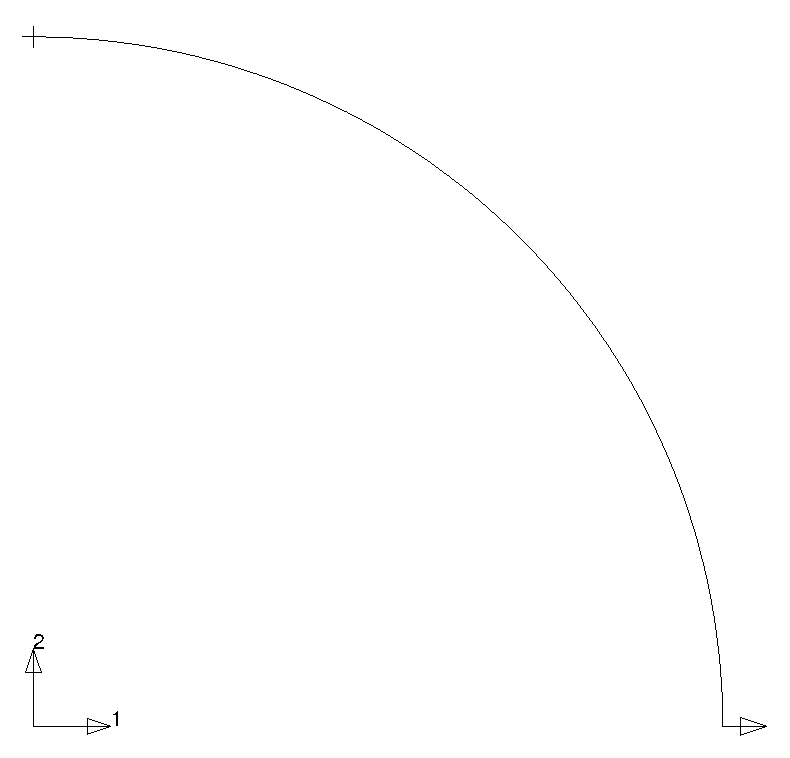
\includegraphics[width=1.6in]{figs/fig7_1} \hfil}
\caption{Curved Beam}
\label{fig71}
\end{figure}

\subsection{The COORdinate Command}
\label{coord}

The coordinates of nodes may be specified using the {\tt COOR}dinate
command.  For example,
the commands to generate polar coordinates for an eleven node mesh of a
circular beam with radius 5 are given by:
\begin{verbatim}
       COORdinates
         1   1     5.0    90.0
        11   0     5.0     0.0
                        ! Termination record
\end{verbatim}
These coordinates may then be converted from polar to Cartesian form
using the {\tt POLA}r command.  For the coordinate input shown above this
is given as:
\begin{verbatim}
       POLAr
         NODES 1   11    1
                        ! Termination record
\end{verbatim}
which converts the nodes 1 to 11 in increments of 1.

After the {\tt COOR}inate command individual records defining each nodal point
and its coordinates are specified as:
\begin{verbatim}
       N, NG, X_N, Y_N, Z_N
\end{verbatim}
where
\begin{center}
\begin{tabular}{ l l }
{\tt N  } & Number of nodal point. \\
{\tt NG } & Generation increment to next node. \\
{\tt X-N} & value of $x_1$ coordinate. \\
{\tt Y-N} & value of $x_2$ coordinate. \\
{\tt Z-N} & value of $x_3$ coordinate. \\
\end{tabular}
\end{center}
It is only necessary to specify the components corresponding to the
spatial dimension of the mesh ({\tt NDM} on the control record).
Thus for 2-dimensional meshes only {\tt X-N} and {\tt Y-N} need be given.

Generation of missing data is performed using data pairs given as:
\begin{verbatim}
       M, MG, X_M, Y_M, Z_M
       N, NG, X_N, Y_N, Z_N
\end{verbatim}
The missing data is generated from {\tt M} to {\tt N} in increments of
{\tt MG}; that is the first generated node will be {\tt M+MG}.  Linear
interpolation of the coordinates is used to define the values for the
generated nodes.  If {\tt MG} is zero no generation is performed.
Nodes may be in either increasing or decreasing order.  The sign
of a non-zero {\tt MG} will be adjusted to ensure that generation is
in the correct direction.

Coordinate data is processed to determine the total number of nodes in a
mesh.
Nodal coordinates may also be defined using the {\tt BLOC}k
or the {\tt BLEN}d commands.

\subsection{The ELEMent Command}
\label{elem}

The {\tt ELEM}ent command may be used to input the list of nodes connected
to an individual element.  For elements where the maximum number of
nodes is less or equal to 13 (i.e., the {\tt NEN} parameter on the
control record), the records following the command are
given as:
\begin{verbatim}
       N, NG, MA, (ND_i, i=1,NEN)
\end{verbatim}
where
\begin{center}
\begin{tabular}{ l l }
{\tt N }  & Number of element. \\
{\tt NG}  & Generation increment for node numbers. \\
{\tt MA}  & Material identifier associated with element. \\
{\tt ND-i} & i-Node number defining element . \\
\end{tabular}
\end{center}
For meshes which have elements with more than 13 nodes on each element,
the sets of records following the command are given as:
\begin{verbatim}
       N, NG, MA, (ND_i, i=1,13)
                  (ND_i, i=14,29)
                  (ND_i, i=30,NEN)
\end{verbatim}
That is, each record must contain no more than 16 items of data as mentioned
in Chapter \ref{record}.

The element numbers following each {\tt ELEM}ent command must be in increasing
numerical order.  If gaps appear in consecutive records
for the number of the element
the missing elements will be generated by adding the generation
value {\tt NG} to each non-zero {\tt ND-i} of the preceding element.  Thus,
the pair of records:
\begin{verbatim}
       M, MG, MA, (MD_i, i=1,NEN)
       N, NG, NA, (ND_i, i=1,NEN)
\end{verbatim}
where {\tt N - M} $> 0$ will generate the records:
\begin{verbatim}
       M+1, -, MA, (MD_i+MG  , i=1,NEN)
       M+2, -, MA, (MD_i+MG*2, i=1,NEN)
       ....
       N-1, -, MA,  ......
\end{verbatim}
until element {\tt N} is reached.

Element data for the mesh for the curved line shown in Figure \ref{fig71}
is given by:
\begin{verbatim}
       ELEMents
         1   1   1   1   2
        10   0   1  10  11
                        ! Termination record
\end{verbatim}
The mesh produced by this set of commands is shown in Figure \ref{fig72}

\begin{figure}[ht!]
\centerline {\hfil 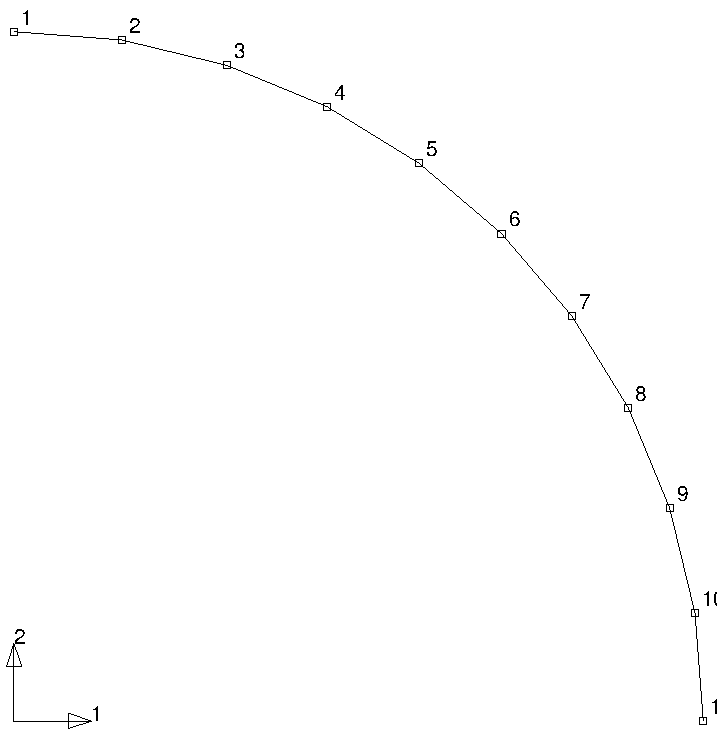
\includegraphics[width=1.6in]{figs/fig7_2} \hfil}
\caption{Mesh for Curved Beam.  10 Elements}
\label{fig72}
\end{figure}

Element data is processed to determine the total number of elements in a mesh.
Element data may also be defined using the {\tt BLOC}k and {\tt BLEN}d commands.

\subsection{The BLOCk Command}
\label{block}

Regular patterns of nodes and element may be input using the
{\tt BLOC}k command.  The block command can input patches of line
elements (truss or frames), triangles or quadrilaterals, or three
dimensional hexahedral (brick) or tetrahedral elements.

The data to input a {\it line} of elements is defined as:
\begin{verbatim}
       BLOCk
         type,r-inc,,node1,elmt1,mat,r-skip
         1,X_1,Y_1,Z_1
            ...
         N,X_N,Y_N,Z_N
                  ! Termination record
\end{verbatim}
The data to input a patch of {\it triangular or quadrilateral}
elements is defined as:
\begin{verbatim}
       BLOCk
         type,r-inc,s-inc,node1,elmt1,mat,r-skip,b-type
         1,X_1,Y_1,Z_1
            ...
         N,X_N,Y_N,Z_N
                  ! Termination record
\end{verbatim}
The data to input a three dimensional block
of {\it hexahedral or tetrahedral} elements are defined as:
\begin{verbatim}
       BLOCk
         type,r-inc,s-inc,t-inc,node1,elmt1,mat,b-type
         1,X_1,Y_1,Z_1
            ...
         N,X_N,Y_N,Z_N
                  ! Termination record
\end{verbatim}
where the parameters are defined as:
\begin{center}
\begin{tabular}{l l}
\it Type  &- Master node coordinate type ({\tt CART, POLA,}\\
\it r-inc &- Number of nodal increments to be generated along \\
          &\quad r-direction of the patch. \\
\it s-inc & - Number of nodal increments to be generated along \\
          &\quad s-direction of the patch. \\
\it t-inc &- Number of nodal increments to be generated along \\
          &\quad t-direction of the patch (N.B. Not input for 2-d). \\
\it Node1 &- Number to be assigned to first generated node in \\
          &\quad patch (default = automatic).  First node is \\
          &\quad located at same location as master node 1. \\
\it Elmt1 &- Number to be assigned to first element generated in \\
          &\quad patch; if zero no elements are generated \\
          &\quad (default = automatic) \\
\it Matl  &- Material identifier to be assigned to all generated elements \\
          &\quad elements in patch (default = 1 or last input value) \\
\it r-skip &- For surfaces, number of nodes to skip between end of \\
          &\quad an r-line and start of next r-line (default = 1) \\
          &\quad (N.B. Not input for 3-d). \\
\end{tabular}
\end{center}

\begin{center}
\begin{tabular}{l l}
\it b-type &=0: 4-node elements on surface patch; \\
           &\qquad 2-node elements on a line; \\
           &=1: 3-node triangles (diagonals in 1-3 direction of block); \\
           &=2: 3-node triangles (diagonals in 2-4 direction of block); \\
           &=3: 3-node triangles (diagonals alternate 1-3 then 2-4); \\
           &=4: 3-node triangles (diagonals alternate 2-4 then 1-3); \\
           &=5: 3-node triangles (diagonals in union-jack pattern); \\
           &=6: 3-node triangles (diagonals in inverse union-jack pattern); \\
           &=7: 6-node triangles (similar to =1 orientation); \\
           &=8: 8-node quadrilaterals ({\it r-inc} and {\it s-inc} must be even \\
           &\qquad numbers);  N.B. Interior node generated but not used; \\
           &=9: 9-node quadrilaterals ({\it r-inc} and {\it s-inc} must be even \\
           &\qquad numbers); \\
           &=10: 8-node hexahedral (bricks).\\
           &=11: 4-node tetrahedra.\\
\end{tabular}
\end{center}

An example mesh input using the {\tt BLOC}k command is the line
elements shown in Figure \ref{fig72}.
For two node elements the necessary data is:
\begin{verbatim}
       BLOCk
         POLAr 10 1 0 0 1
         1   5.0   90.0
         2   5.0    0.0
                  ! Termination record
\end{verbatim}
When using the {\tt BLOC}k command one may enter zero for the
{\it Node1} and {\it Elmt1} parameters.
Values for the node and element numbers will then be automatically generated
in the sequence data is input.  Restrictions apply when mixing {\tt BLOC}k
or {\it BLEN}d options with the {\tt ELEM} option where numbers are required.

While polar coordinates
may be used directly as input for the block master coordinates using the
{\tt POLA}r option,
the actual nodal coordinates generated will be converted automatically
from polar to Cartesian coordinates using the current {\tt SHIF}t values
for $x_0$, $y_0$, and $z_0$.
With this option it also is not necessary to know the numbers for the
generated nodes, as was required to use the {\tt COOR}\-dinate and
{\tt POLA}r commands.
For three dimensional problems the {\tt POLA}r option becomes a cylindrical
coordinate transformation.

\subsection{The BLENd Command}
\label{blend}

A block of nodes and elements also may be generated using a
blending function approach
(e.g., see ~\cite{zt1}, pp 181 ff. or similar information in ~\cite{zt1n}).
In {\sl FEAPpv} the blending function meshes are created from a set of control
points - call super-nodes - ({\tt SNOD}e command),
edges ({\tt SIDE} command) and
the {\tt BLEN}d command.  Meshes may be created as {\tt SURF}aces in
two and three dimensions or as {\tt SOLI}ds in three dimensions.  The
two dimensional blended mesh shown in Figure \ref{figb1} has three straight
sides and one circular arc side.  The spacing along each side is uniform,
thus only end points are required to specify the control points.
For non-uniform spacing additional control points may be given
for edges.  To construct this mesh the coordinates for the five
super-nodes, the one arc edge, and the vertices for the blend
region must be specified as shown in Figure \ref{figb2}.

\begin{figure}[ht!]
\centerline {\hfil 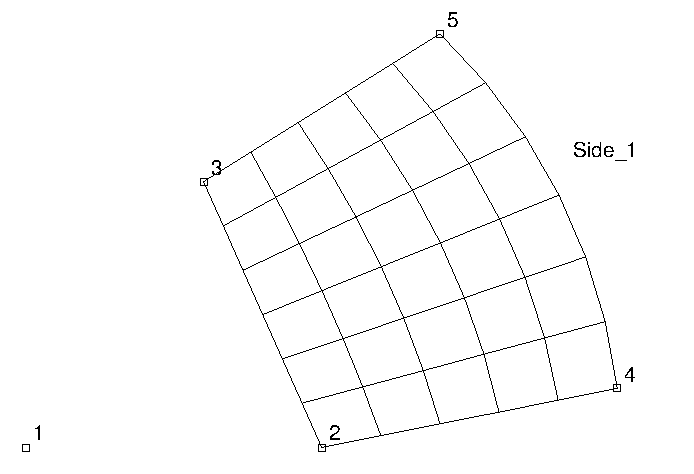
\includegraphics[width=3.6in]{figs/figb1} \hfil}
\caption{Two-dimensional Blended Mesh}
\label{figb1}
\end{figure}

\begin{figure}[ht!]
\begin{verbatim}
       SNODes
         1  0   0
         2  5   0
         3  3   4.5
         4 10   1
         5  7   7
                   ! Blank termination record
       SIDE
         POLAr  4  5  1
                   ! Blank termination record
       BLENd
         SURFace  5  6  0  0  1
          2  4  5  3
                   ! Blank termination record
\end{verbatim}
\caption{Two-dimensional blended mesh data}
\label{figb2}
\end{figure}

The coordinates for super-nodes {\it always} are given in Cartesian form.
Also, only the edges for non-straight or non-uniformly spaced increments
need be given.  {\sl FEAPpv} will automatically add all
straight uniformly spaced edges not given as input data.
The specification of edges using the {\tt SIDE} command is given by the
general form:
\begin{verbatim}
       Type,V1,V2,V3,....,V14
\end{verbatim}
where {\tt Type} is the geometric type for the
side, and {\tt Vi} are a list of values.
Edges are one of three different {\tt Type}s:
\begin{enumerate}
\item
{\tt Type = CARTesian}: For Lagrange interpolation in Cartesian coordinates.
The {\tt Vi} values are the numbers of super-nodes used for the interpolation

$$\B{x}(\xi) ~=~ \sum_i L_i(\xi) \B{x}_{Vi}$$
where $L_i(\xi)$ are Lagrange interpolation polynomials in the natural
coordinate $\xi$.

\item
{\tt Type = POLAr}: For Lagrange interpolation in polar coordinates.  The
interpolations are given as:

$$r(\xi) ~=~ \sum_i L_i(\xi) r_{Vi}$$
$$\theta(\xi) ~=~ \sum_i L_i(\xi) \theta_{Vi}$$
where the radii $r_{Vi}$ use the last specified super-node number in the
list for {\tt Vi} as the location of their origin.

\item
{\tt Type = SEGMent}: For multiple straight segments with uniform increments
on each segment.  In this form the odd entries {\tt V1, V3, V5, ...}
are super-node numbers and the even entries {\tt V2, V4, V6, ...}
are the number of increments between the adjacent super-nodes.
\end{enumerate}

For two-dimensional blended meshes the {\tt SURF}ace option is used and 
four vertex super-nodes specify the orientation of the region.
The super-nodes must be given as an anti-clockwise sequence (right hand
rule).
For three-dimensional blended meshes either the {\tt SURF}ace or the
{\tt SOLI}d option may be used to generate the mesh region.  For the
{\tt SURF}ace option the ordering is any contiguous four super-node sequence.
For the {\tt SOLI}d option the vertex order is identical to that for the
8-node {\tt BLOC}k command: That is, number the super-nodes by right hand rule
with the first four nodes on the {\it bottom} face and the last four
on the {\it top} face.
The number of generation increments and other parameters are 
given in Table \ref{tabb1} for surface generations and in Table \ref{tabb2}
for solid generations.

\begin{table}[ht!]
\begin{center}
\begin{tabular}{l l}
\it Type  &- Blend type ({\tt SURF}ace. \\
\it 1-inc &- Number of nodal increments to be generated along \\
          &\quad 1-2 edge. \\
\it 2-inc & - Number of nodal increments to be generated along \\
          &\quad 2-3 edge. \\
\it Node1 &- Number to be assigned to first generated node in \\
          &\quad patch (default = automatic).  First node is \\
          &\quad located at same location as master node 1. \\
\it Elmt1 &- Number to be assigned to first element generated in \\
          &\quad patch; if negative no elements are generated \\
          & (default = automatic) \\
\it Matl &- Material identifier to be assigned to all generated elements \\
         &\quad elements in patch (default = 1) \\
\end{tabular}
\end{center}
\caption{Surface Blend Parameters}
\label{tabb1}
\end{table}
\begin{table}[ht!]
\begin{center}
\begin{tabular}{l l}
\it type  &- Blend type {\tt SOLI}d. \\
\it 1-inc &- Number of nodal increments to be generated along \\
          &\quad 1-2 edge. \\
\it 2-inc & - Number of nodal increments to be generated along \\
          &\quad 2-3 edge. \\
\it 3-inc &- Number of nodal increments to be generated along \\
          &\quad 1-5 edge. \\
\it Node1 &- Number to be assigned to first generated node in \\
          &\quad patch (default = automatic).  First node is \\
          &\quad located at same location as master node 1. \\
\it Elmt1 &- Number to be assigned to first element generated in \\
          &\quad patch; if negative no elements are generated \\
          &\quad (default = automatic) \\
\it Matl  &- Material identifier to be assigned to all generated elements \\
          &\quad elements in patch (default = 1) \\
\end{tabular}
\end{center}
\caption{Three-dimensional Solid Blend Parameters}
\label{tabb2}
\end{table}

A blended region for a three dimensional mesh is shown in Figure \ref{figb3}
and generated using the data shown in Figure \ref{figb4}.

\begin{figure}[ht!]
\centerline {\hfil 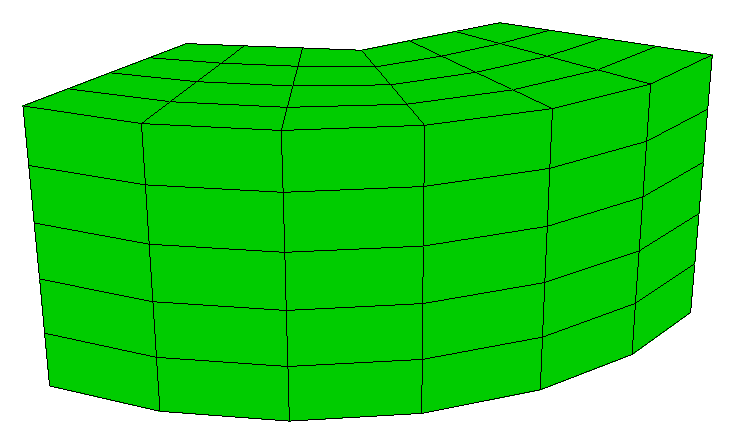
\includegraphics[width=2.5in]{figs/figb3a} \hspace{0.5in}
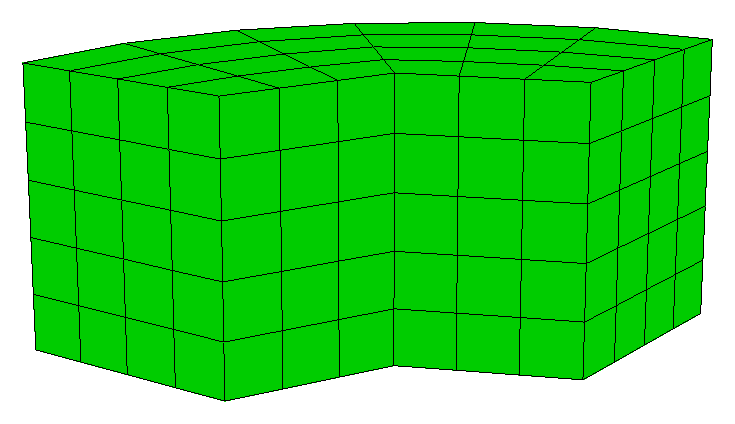
\includegraphics[width=2.5in]{figs/figb3b} \hfil}
\caption{Three-dimensional Blended Mesh}
\label{figb3}
\end{figure}

\begin{figure}[ht!]
\begin{verbatim}
       SNODes
         1    0   0  0
         2   10   0  0
         3    0  10  0
         4    5   0  0
         5  3.5 3.5  0
         6    0   5  0
         7    0   0  6
         8   10   0  6
         9    0  10  6
        10    5   0  6
        11  3.5 3.5  6
        12    0   5  6
                   ! Blank termination record
       SIDEs
         POLA   2  3  1
         SEGM   4  3  5  3  6
         POLA   8  9  7
         SEGM  10  3 11  3 12
                   ! Blank termination record
       BLEND
         SOLID  6  4  5
          2  3  6  4  8  9 12 10
                   ! Blank termination record
\end{verbatim}
\caption{Three-dimensional blended mesh data}
\label{figb4}
\end{figure}

Nodes and elements may be generated using a combination of the
above schemes.  Thus, it is possible to mix the {\tt BLOC}k and
{\tt BLEN}d options with the
{\tt COOR}d\-in\-ate and {\tt ELEM}\-ent commands to generate the mesh.
Furthermore,
the mesh may be described using any of the coordinate systems as inputs
and subsequently (or in the case of the {\tt BLOC}k 
and {\tt BLEN}d options simultaneously)
converting the input and/or generated coordinates to Cartesian coordinate
values using the {\tt POLA}r command.
